\section{2009 - PHYSICS 2A ALTERNATIVE A PRACTICAL}

\begin{enumerate}
\item[1.] In this experiment you are required to find the relationship between the length of a simple pendulum and its period. Proceed as follows:
\begin{itemize}
\item[(a)] Suspend a simple pendulum of length L = 100 cm. Displace the pendulum through a small angle so that it swings parallel to the edge of the bench or table, determine the time for 20 oscillations. Continue reducing the length of the pendulum by 10 cm each time and obtain a total of six readings.
\item[(b)] Record your readings in a table as shown below.


\begin{tabular}{|p{2.5cm}|p{2.5cm}|p{2.5cm}|p{2.5cm}|p{2.5cm}|} \hline
Length of pendulum L (cm) & Log$_{10}$L & Time for 20 oscillations & Period T & Log$_{10}$T \\ \hline
&&&& \\ 
&&&& \\ 
&&&& \\ 
&&&& \\ 
&&&& \\ 
&&&& \\ 
&&&& \\ 
&&&& \\ \hline
\end{tabular}\\[10pt]

\noindent Assuming that T $ \propto $ L$^a$, we have T = $k$L$^a$ and taking logarithms to base ten on both sides we get $\log_{10}$T = $a\log_{10}$L + $\log_{10}k$.

\begin{itemize}
\item[(i)] Plot a graph of $\log_{10}$T (vertical axis) against $\log_{10}$L (horizontal axis) hence determine the values of $a$ and $k$ each correct to one decimal place.
\item[(ii)] From your answer in (i) above write down the values of $a$ and $k$ each in the form of $\cfrac{b}{c}$ where $b$ and $c$ are integers (i.e. whole numbers).
\item[(iii)] From the assumption and your answer in (ii) deduce the form of the equation governing the motion of the simple pendulum.
\end{itemize}

\end{itemize}
\end{enumerate}
\flushright \textbf{(25 marks)}


\begin{enumerate}
\item[2.] The aim of this experiment is to determine the refractive index $\eta$ of a given glass block.

\begin{center}
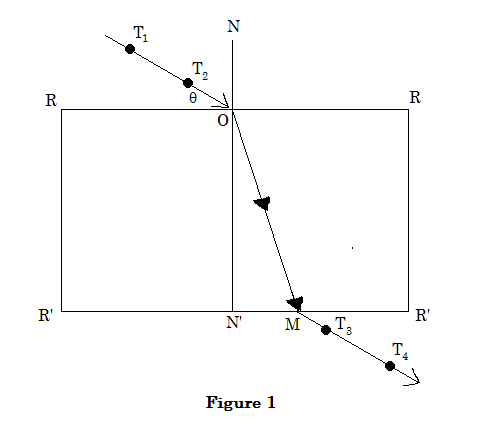
\includegraphics[width=8cm]{./img/2009-2-alt.png}
\end{center}

Place the rectangular glass block on the white paper on a drawing board. Using a pencil trace the outline of the block. Remove the glass block and draw a normal NOM near the left end of the block (Figure 1).\\[10pt]

\noindent Using a protractor and a pencil measure $\theta = 20^\circ$, draw a line making the angle $20^\circ$ with the surface RR of the block. Erect two pins T$_1$ and T$_2$ on this line and at a suitable distance from one another. Return the block and erect the pins T$_3$ and T$_4$ at positions such that they lie in a straight line with pins T$_1$ and T$_2$ as seen through the block. Now remove the block and draw a complete path of the ray (Figure 1).\\[10pt]

\noindent Measure the length MN$'$ and ON$'$: Repeat the procedure for values of $\theta = 30^\circ, 40^\circ$ and $60^\circ$ respectively. In each case make a drawing on a fresh part of the drawing paper.

\begin{itemize}
\item[(a)] Record the values of $\theta$, MN$'$, ON$'$, $\cfrac{\text{MN}'}{\text{ON}'}$ and $\cos \theta$ in a tabular form.
\item[(b)] Plot a graph of $\cfrac{\text{MN}'}{\text{ON}'}$ against $\cos \theta$.
\item[(c)] Find the slope $G$ of the graph.
\item[(d)] Calculate the value of the refractive index $\eta$; given that $G = \cfrac{1}{\eta}$.
\item[(e)] State two sources of errors. \hfill \textbf{(25 marks)}
\end{itemize}

\end{enumerate}


\begin{enumerate}
\item[3.] The aim of this experiment is to verify Ohm's Law.

\begin{center}
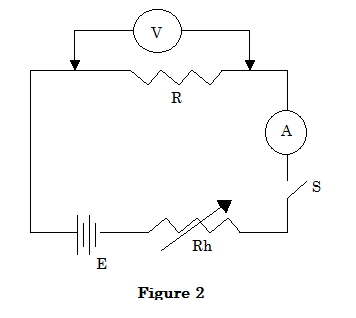
\includegraphics[width=7cm]{./img/2009-3-alt.png}
\end{center}

\begin{itemize}
\item[(a)] Set up the apparatus as shown on Figure 2, close switch S. Adjust the Rheostat Rh by sliding slowly from one end, read and record the value V of the voltmeter and current I of the ammeter.
\item[(b)] Repeat the experiment by changing the Rheostat slider to obtain about five pair of readings.\\[10pt]

\textbf{NB:} Adjust the Rheostat until when the pointer is exactly on the division of the metre scale.\\[10pt]

Table of results\\[10pt]
\begin{tabular}{|c|c|c|c|c|c|c|c|}\hline
V (V)&&&&&&&\\ \hline
I (A)&&&&&&& \\ \hline
\end{tabular}

\item[(c)] Plot a graph of V (vertical axis) against I (horizontal axis).
\item[(d)] 
\begin{itemize}
\item[(i)] Find the slope of the graph.
\item[(ii)] What is the relation between V and I?
\item[(iii)] Find the resistance R. \hfill \textbf{(25 marks)}
\end{itemize}
\end{itemize}

\end{enumerate}
\flushleft
